\chapter{Konzepte}
\label{chap:konzepte}
Wie bereits in dem vorangegangenen Kapitel \emph{\nameref{sec:Vorgehensweise}} hervorgehoben wurde, bildet die Entwicklung und Ausarbeitung von Konzepten einen essenziellen Eckpfeiler bei der Bewältigung und Lösungsfindung für komplexe Probleme. Im nachfolgenden Abschnitt wird eine ausführliche Vorstellung und Evaluation der erarbeiteten Konzepte präsentiert. Dabei liegt der Fokus darauf zu ergründen, welche Konzepte das Potenzial besitzen, weiterverfolgt zu werden, um die spezifische Herausforderung zu meistern. Besondere Aufmerksamkeit gilt hierbei der grundlegenden Idee jedes Konzeptes sowie der detaillierten Darlegung, wie jedes einzelne Konzept dazu beitragen kann, dynamische Preisgestaltung für ein Hotel auch ohne vorhandene Daten zu generieren
\newline
\newline
Ziel dieses Kapitels ist es einen umfassenden Überblick über die Konzepte zu geben, ihre Relevanz für die Forschung zu betonen und den Weg für die darauffolgenden Analysen und Schlussfolgerungen zu ebnen.

\section{Hotel Daten von vielen Hotels}
\label{sec:all_Hotels}
Das Konzept \emph{Hotel Daten von vielen Hotels} verfolgt die grundlegende Idee, sämtliche bis dato gesammelten Hoteldaten zu konsolidieren und ein umfassendes, übergeordnetes Modell des maschinellen Lernens zu entwickeln.
\newline
\newline
Die bereits vorhandenen Daten aus zahlreichen Hotels bildet die Basis für den Aufbau eines solchen Modells. Dieses Vorhaben sieht vor, das bereits existierende RevPAR-Modell zu modifizieren und zu erweitern. Zunächst wird angestrebt, alle Hotels in eine vergleichbare Form zu bringen. Eine mögliche Herangehensweise hierbei ist die Definition bestimmter Hotelmerkmale und ihre Auflistung als Vektor, um eine Vergleichbarkeit zu ermöglichen.
\newline
\newline
Im nächsten Schritt ist eine Anpassung des RevPAR-Modells erforderlich, da dieses normalerweise auf Buchungsdaten basiert. Für Hotels ohne historische Buchungsdaten ist es offensichtlich nicht möglich, diese als Features zu verwenden, da sie schlichtweg nicht verfügbar sind. Stattdessen sollen die charakteristischen Merkmale jedes Hotels dem jeweiligen RevPAR zugeordnet werden.
\newline
\newline
Sobald das RevPAR-Modell entsprechend umstrukturiert ist, können sämtliche Hotels in der Datenbank als Datensätze dem Modell zugeführt werden. Falls ein Hotel ohne vergangene Buchungsdaten auftaucht, können basierend auf seinen charakteristischen Eigenschaften Prognosen über den zu erwartenden RevPAR getroffen werden. In diesem Szenario muss das Hotel lediglich, wie alle anderen Hotels auch, eine Zuordnung zwischen dem RevPAR und dem tatsächlichen Preis festlegen.
\newline
\newline
Die Aufmachung dieses Konzeptes soll im folgenden Schaubild nochmal Bildlich verdeutlicht werden:
\begin{figure}[h]
    \centering
    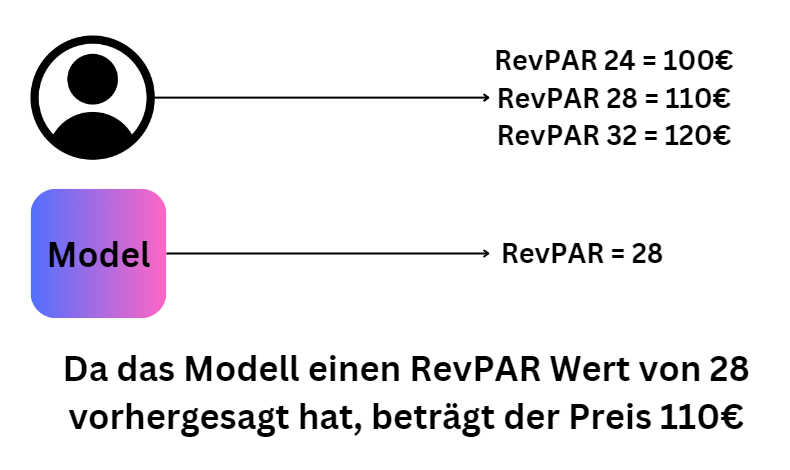
\includegraphics[width=0.5\textwidth, center]{RevPAR_all.png}
    \caption[RevPAR-Modell Vorgehen]{RevPAR-Modell Vorgehen}
    \label{img:all_hotels}
\end{figure}

Dieser Ansatz zielt darauf ab, eine umfassende Verwendung der vorhandenen Daten zu ermöglichen und somit auch für Hotels ohne historische Buchungsdaten eine Prognose des RevPAR auf der Grundlage ihrer individuellen Eigenschaften zu ermöglichen.
\section{Mitbewerber Modell}
\label{sec:Mitbewerber}
Die grundlegende Idee des Konzeptes: Mitbewerber Modell ist es, die Daten von der Konkurrenz zu benutzen um daraufhin Preisvorschläge zu generieren. 
\newline
\newline
Durch dritt Anbieter wie \emph{HQ-Revenue} können Konkurrenzdaten genutzt werden um ein Modell aufzubauen. HQ-Revenue ist ein Anbieter, welcher Internetseiten wie Bookings.com oder trivago \emph{scraped} um an Hotelpreise oder andere Daten zu kommen. Dabei gibt es viele verschiedene Vorgehensweisen um Preise für ein Hotel ohne Vergangenheitsdaten zu entwickeln. Ein Primitiver Ansatz dabei wäre es, wenn alle Preise von den Konkurrenten genommen werden und damit der Durchschnitt ermittelt wird. Dies hat natürlich nichts mit Machine Learning oder geschweige denn Data Science zu tun aber es wäre ein Ansatz der Verfolgt werden könnte. 
\newline
\newline
Dieser Ansatz birgt jedoch eine Problematik: Nicht jeder Kunde von happyhotel hat auch automatisch Konkurrenzdaten zur Verfügung, diese müssen noch dazu gebucht werden. Deswegen wird folgender Ansatz verfolgt. 
\newline
\newline
So wie im vorherigen Konzept \emph{\nameref{sec:all_Hotels}} werden auch hier die Hotels in eine Vergleichbare Form gebracht. Das Ziel ist es dann ein oder mehrere Hotels zu finden, die vermeintlich ähnlich sind. Sobald ein oder mehrere ähnliche Hotels gefunden worden sind, können die Konkurrenzdaten von den ähnlichen Hotels genutzt werden. 
\newline
\newline
Als Zielvariable des Modells werden dann die Preise des ähnlichsten Hotels verwenden.  Jedoch sollen hierbei die Preise von den Konkurrenten und von dem ähnlichsten Hotel nicht einfach so benutzt werden, sondern lediglich das Verhältnis. Die Preise sollen anhand von dem Durchschnittlichen Preis in Verhältnis gebracht werden und dieses Verhältnis soll vorhergesagt werden. 
\newline
\newline 
Das Hotel ohne Vergangenheitsdaten muss in diesem Fall dann einen Durchschnittlichen Preise angeben, anhand dessen mit dem vorhergesagten  Verhältnis der tatsächliche Preis abgeleitet werden kann. Dies soll im folgenden Schaubild noch einmal dargestellt werden:
\begin{figure}[h]
    \centering
    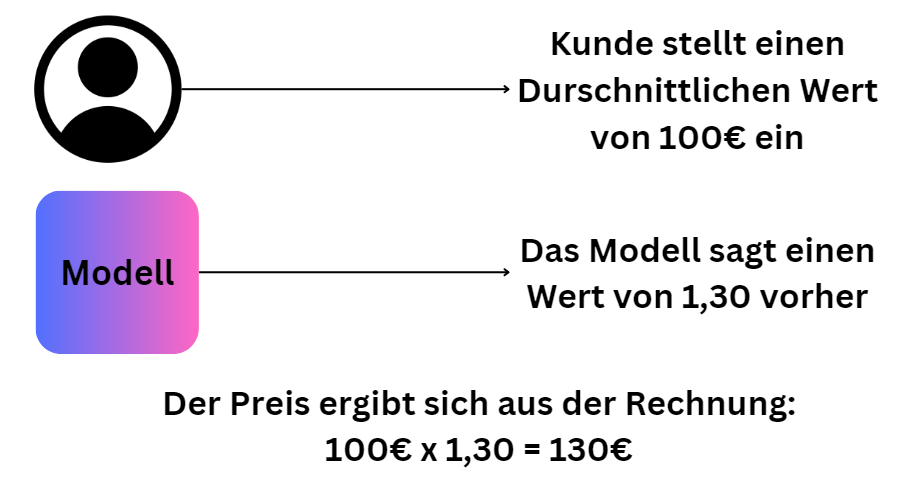
\includegraphics[width=0.5\textwidth, center]{Mitbewerber_model.png}
    \caption[Mitbewerber Modell]{Mitbewerber Modell}
    \label{img:all_hotels}
\end{figure}

\section{Ähnliche Hotels}
\label{sec:aehnliche_hotels}
Dieses Konzept der \emph{Ähnlichen Hotels} verschmilzt in gewisser Weise die Ideen der beiden Konzepte \emph{Mitbewerber Modell} und \emph{Hotel Daten von vielen Hotels}. Dieser Ansatz zielt darauf ab, ähnliche Hotels zu identifizieren und basierend auf den Daten dieser Hotels ein Modell zu entwickeln.
\newline
\newline
Im Gegensatz zum Konzept \emph{Hotel Daten von vielen Hotels} besteht bei diesem Ansatz die Möglichkeit, konkrete Buchungsdaten der jeweiligen Hotels zu verwenden. Die primäre Herausforderung liegt jedoch darin, die ähnlichsten Hotels zu identifizieren. Nachdem diese ähnlichen Hotels ausfindig gemacht wurden, kann das bereits vorhandene Modell \emph{Kombination aus RevPAR und Buchungskurve} ohne jegliche Anpassungen genutzt werden.
\newline
\newline
Dieses Modell wird dann, ähnlich wie bei anderen Hotels, mit den Buchungsdaten der zugrunde liegenden ähnlichen Hotels gefüttert, um Preise zu generieren. In diesem Szenario muss der Kunde lediglich eine Zuordnung zwischen dem RevPAR-Wert und dem konkreten Preis des Hotels festlegen.
\newline
\newline
Diese Vorgehensweise kombiniert die Vorteile beider vorherigen Konzepte, indem er sowohl auf die Ähnlichkeitsfindung zwischen Hotels, als auch auf die Nutzung spezifischer Buchungsdaten abzielt. Durch die Verwendung vorhandener Modelle ohne umfangreiche Modifikationen können so gezielt Preisvorhersagen für ähnliche Hotels generiert werden.
\section{Synthetische Daten erstellen}
\label{sec:Synthetische}
Das Konzept der \emph{Erstellung synthetischer Daten} markiert einen innovativen Ansatz innerhalb der Konzepte und weicht von den bisherigen Strategien ab. Dieser Ansatz verfolgt die Idee, ein Modell mit sämtlichen verfügbaren Daten zu trainieren und darauf aufbauend synthetische zukünftige Daten zu generieren. Ziel ist es, eine Art Simulation zu erstellen, die den Buchungsverlauf eines Hotels nachbildet.
\newline
\newline
Mittels dieser Simulation wird angestrebt, Vorhersagen darüber zu treffen, wie viele Buchungen für bestimmte Zimmerkategorien an bestimmten Tagen eingehen werden. Dadurch soll die Möglichkeit geschaffen werden, einen dynamischen Preis entsprechend dem erwarteten Buchungsverlauf zu gestalten.
\newline
\newline
Die Grundidee hinter dieser Vorgehensweise liegt in der Schaffung eines virtuellen Modells, welches basierend auf vergangenen Daten und Mustern potenzielle zukünftige Buchungen simuliert. Hierbei sollen verschiedene Szenarien durchgespielt werden, um die wahrscheinlichsten Buchungstrends abzuschätzen, und somit einen fundierten Ansatz für die dynamische Preisgestaltung zu generieren.
\section{Evaluation}
\label{sec:eval_konzept}
Nachdem nun die ausgearbeiteten Konzepte vorgestellt wurden, gilt es diese zu Bewerten um festzulegen mit welchen Konzepten fortgefahren werden soll. Jedes der vorgestellten ist auf seine Art valide und hat auch Berechtigung verfolgt zu werden. Um deshalb entscheiden zu können, welches Konzept überhaupt nachgegangen werden soll oder in welcher Reihenfolge die Konzepte ausprobiert werden sollen, werden die Konzepte nach den folgenden Kriterien bewertet:
\begin{itemize}
    \item Aufwand
    \item Erfolgswahrscheinlichkeit
    \item Impact
\end{itemize}
Aufwand und Erfolgswahrscheinlichkeit sind selbsterklärend. Der Impact bezieht sich darauf, in wie fern happyhotel im generellen von dem Konzept profitieren könnte und ob das Konzept nicht auch für schon vorhandene Kunden eingesetzt werden könnte.
\newline
\newline
Jedes Konzept kann bei jedem Kriterium eine Zahl zwischen 1 bis 5 erzielen, wobei 5 das Beste und 1 das Schlechteste in dem jeweiligen Kriterium bedeutet. Die Ergebnisse der Evaluation sind wie folgt in der Tabelle dargestellt:
\begin{table}[ht]
    \centering
    \begin{tabularx}{\textwidth}{|d|c|c|c|c|}
        \textbf{Konzepte} & \textbf{Aufwand} & \textbf{Erfolgsw.} & \textbf{Impact} & \textbf{Result} \\
        \hline
        Daten von vielen Hotels & 4       & 4            & 4      & 12 
        \\\rowcolor{Gray}
        Mitbewerber             & 4       & 3            & 3      & 10                \\
        Ähnliche Hotels         & 4       & 5            & 4      & 13  
        \\\rowcolor{Gray}
        Synthetischen Daten     & 1       & 3            & 5      & 9   \\
    \end{tabularx}
    \caption[Evaluierung der Konzepte]{Evaluierung der Konzepte}
    \label{table:eval_kozepts}
\end{table}

Nach der Evaluierung wurde bestimmt, dass das Konzept \emph{\nameref{sec:aehnliche_hotels}} das größte Potenzial hat und soll dementsprechend auch verfolgt werden. Je nach Zeit und Ergebnisse werden die Konzepte \emph{\nameref{sec:Mitbewerber}} und \emph{\nameref{sec:all_Hotels}} auch verfolgt und evaluiert werden. Die Erstellung einer Simulation durch Synthetische Daten ist auch ein sehr interessantes Konzept, würde aber im rahmen dieser Thesis zu weit gehen.